\chapter{Analytical Model}
\label{ch:analyticalmodel}
\textit{This chapter intends to explain the calculation of the critical current in different SNS junctions. For this purpose, a quasiclassical transport theory is used and its foundations are explained in the first section. This technique is then employed for a clean SNS junction, and an expression for the Josephson current is found. In the following section, the calculations used for the clean setup are extended for the more sophisticated quantum point contact (QPC) and here as well, the current for the QPC-gated junction is found.}

\section{Foundation of the quasiclassical model}
This section explains preliminary assumptions made to describe the current in a SNS junction. The aim is to express the current through the junction using a quasiclassical approach. Essentially, this means that the Andreev bound states are associated with straight trajectories connecting the superconducting leads. The superconducting current density is then expressed in terms of these trajectories.
\begin{figure}[h]
\centering	
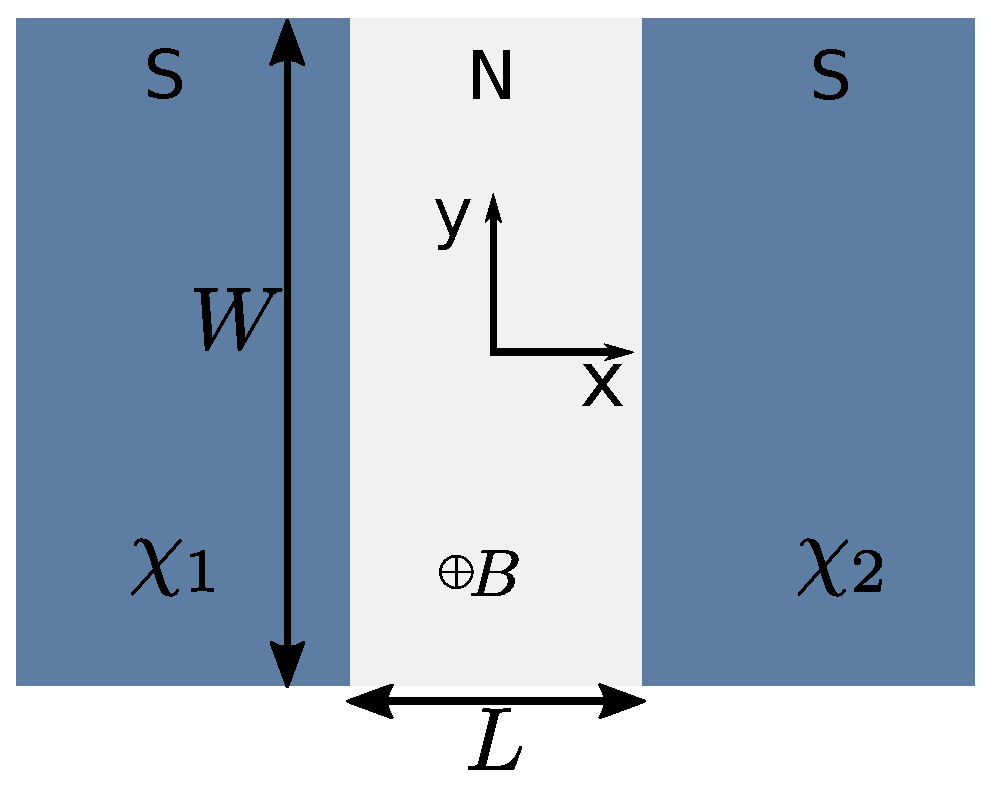
\includegraphics[width=0.6\textwidth]{figure/analyticalmodel/sns_junction}
\caption{Schematic representation of a short and wide SNS junction.}
\label{fig:sns_schematic}
\end{figure}
The two dimensional junction, a schematic is shown in fig \ref{fig:sns_schematic}, is a short and wide junction with width $W$ and length $L$, where $W \gg L$. The NS-interfaces are parallel to the $y$-axis and are placed at $x = \pm L/2$. Each of the superconducting leads has a phase $\chi_{1}$ and $\chi_{2}$, and the overall phase difference is $\chi = \chi_{1} - \chi_{2}$. The superconducting gap parameter is only present in the superconducting leads. Close to the interface, $\Delta$ begins to decay on a length scale of the superconducting coherence length $\xi_0$  into the normal region. For the following calculations, this effect is neglected and a step-like behavior is assumed for the superconducting gap parameter.
\begin{equation}
\Delta\left( x \right) = |\Delta| e^{\chi_1} \Theta\left(-L/2 -x \right) + |\Delta| e^{\chi_2} \Theta\left(x-L/2 \right) 
\label{eq:gap_parameter}
\end{equation}
We consider the low temperature limit, where the thermal length scale of the system is larger than the sample length:
\begin{equation}
L_T = \hbar v_F / k_B T \gg L
\end{equation}
The considered sample is ballistic, which means the fermi wavelength $\lambda_F$ is smaller than the sample length $L$. It has the BCS coherence length $\xi = \hbar v_F / \pi \Delta$, where $\xi$ is much larger than the Fermi velocity $\xi \gg v_F$ 
\textbf{TODO: (in order to induce superconductivity in the system?)}. 
The relation between the coherence length $\xi$ and the sample length $L$ determines if the considered junction is a \textit{short} or a \textit{long} junction:
\begin{eqnarray*}
\xi \ll L \quad \rightarrow \quad \text{long junction} \quad \rightarrow \quad \text{many Andreev levels} \\ 
\xi \gg L \quad \rightarrow \quad \text{short junction} \quad \rightarrow \quad \text{one Andreev level} 
\end{eqnarray*}
\textbf{TODO: replace equation above with good picture (E < delta, andreec levels...)}\\
\textbf{TODO stimmt das oben? Es sollte einen Zusammenhang primaer mit Energie, nicht mit sample size geben...}
The presence of the magnetic field in the normal region of the sample will lead to a bending of the trajectories due to the Lorentz force. Depending on the strength of magnetic field $B$ and the Fermi velocity, the radius of this curve is 
\begin{equation}
r_B = \frac{m^* v_F}{e B}
\end{equation}
%TODO check if correct!
In order to justify the assumption of straight trajectories, either the magnetic field has to be weak enough, or the Fermi velocity (wavelength) has to be large (short) enough. Then, the cyclotron radius $r_B$ is larger than the sample size $L$ and the ass straight trajectories are a valid assumption. 

\section{Plane setup: calculation of current}
%TODO Re-calculate current from Glazman
To derive the current for the SNS setup depicted in figure \ref{fig:sns_schematic}, we start by writing down the Bogoliubov-de-Gennes Hamiltonian for this system.
\begin{equation}
\begin{pmatrix}
-\frac{\hbar^2}{2m} \nabla^2 - \epsilon_F & \Delta(x) \\
\Delta^*(x) & \frac{\hbar^2}{2m} \nabla^2 + \epsilon_F 
\end{pmatrix}
\begin{pmatrix}
\psi_e \\
\psi_h
\end{pmatrix} = E 
\begin{pmatrix}
\psi_e\\
\psi_h
\end{pmatrix}
\end{equation}
The Hamiltonian above uses eq. (\ref{eq:gap_parameter}) for the spatially dependent superconducting gap parameter $\Delta(x)$. The eigenvalue problem has two solutions
\begin{equation}
\epsilon_{\pm} = \frac{\hbar^2 k^2_{\pm}}{2m} = -\epsilon_F - \sqrt{E_k^2 - |\Delta|^2}
\end{equation}
%The corresponding wavefunction (according to Glazman paper):
%\begin{equation}
%\psi_e^{n, \pm} = \frac{1}{\sqrt[WL]{}}
%\end{equation}
%TODO calculate current and wavefunctionsx
\textbf{TODO: Hier fehlt die Herleitung f\"ur Wellenfunktionen, Ausdruck f\"ur den Strom etc.!}
Current density for short and long junction limit: 
In the short junction limit the current density can be derived from the scattering matrix formalism and it reads
\begin{equation}
\mathcal{J}^s (\chi) = \frac{\mathcal{T} \sin \chi}{\sqrt{1 - \mathcal{T} \sin^2 \frac{\chi}{2}}}
\end{equation}
$\mathcal{T}$ is the transmission coefficient that describes the transmission through a channel (each channel corresponds to a eigenvalue of the scattering matrix.
The current density for the long junction limit is
\begin{equation}
\mathcal{J}(\chi) = \sum_{k = 1}^{\infty} \frac{(-1)^{k+1}}{k} \sin( k \chi).
\end{equation}
\begin{figure}
\centering
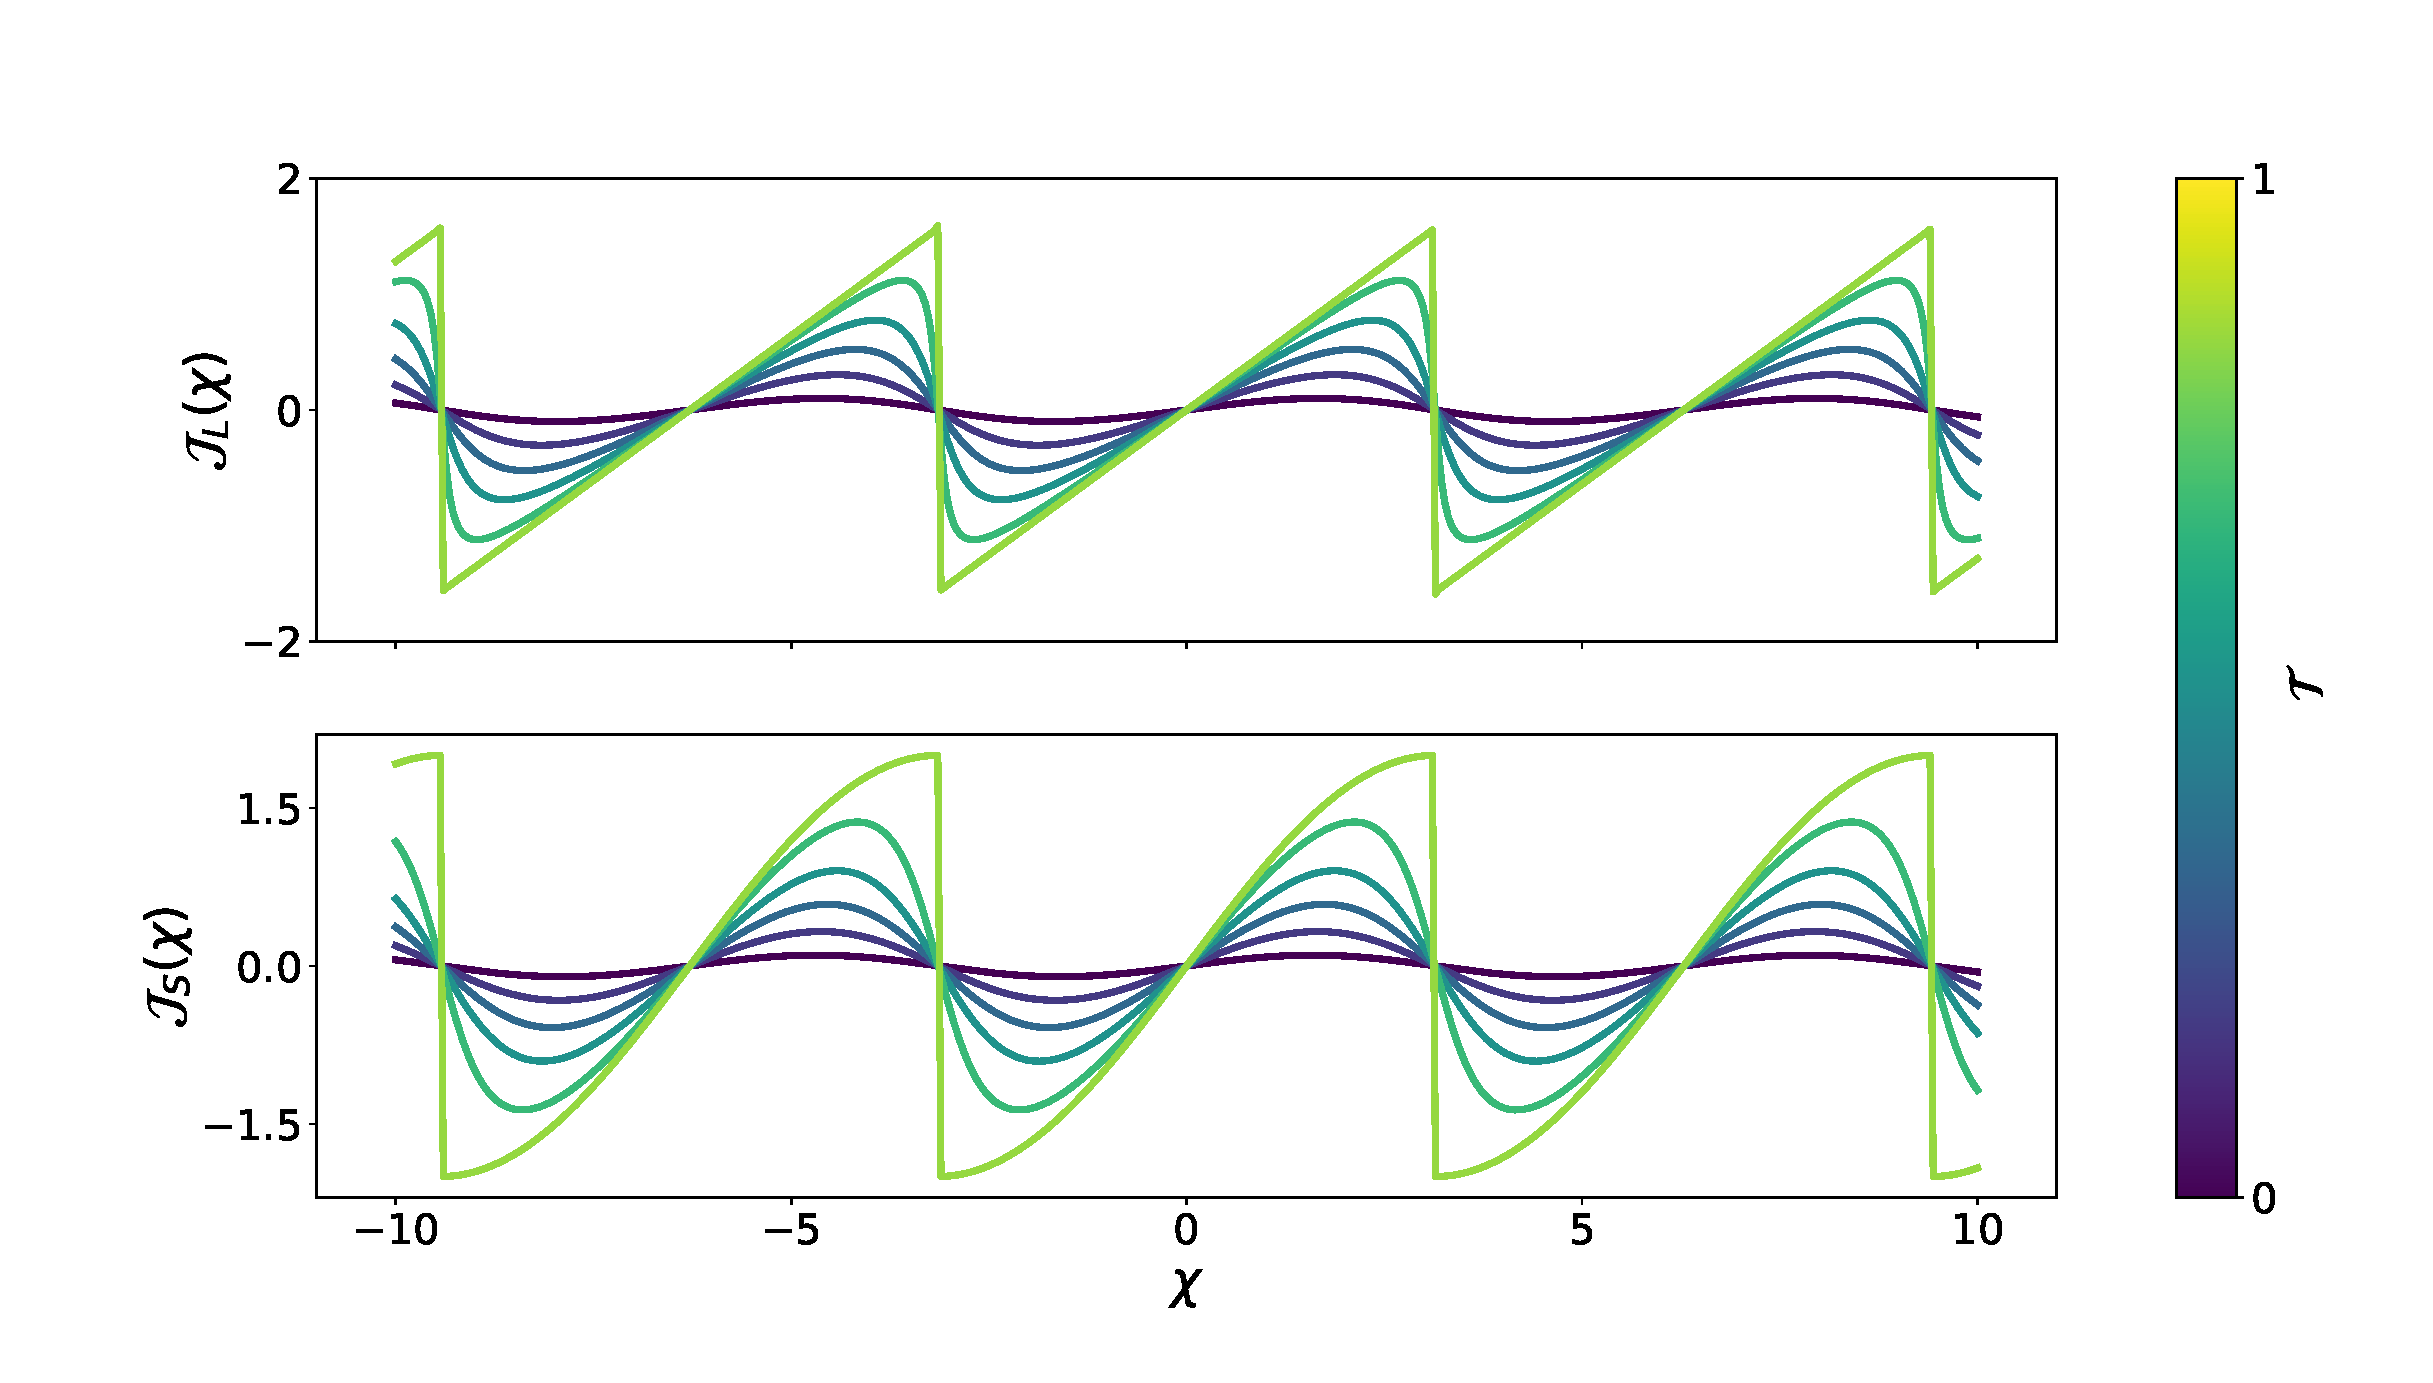
\includegraphics[width=\textwidth]{figure/analyticalmodel/current_density_all}
\caption{Short and long junction current density}
\label{fig:current_density}
\end{figure}
Figure \ref{fig:current_density} shows a plot of both short and long junction limit current densities. They differ for a large transmission coefficient $\mathcal{T} \simeq 1$, where in the long junction limit we observe a sawtooth like shape and in the short junction limit we have a sinusoidal shape.\\
A trajectory connecting the superconducting interfaces can be parametrized by 
\begin{equation}
\tan \theta = \frac{y_2 - y_1}{L}
\label{eq:parametrization}
\end{equation}
with $\theta$ being the angle between the trajectory and the x-axis.\\ \textbf{TODO: figure!}\\ Using the current density the Josephson current at zero magnetic field ($\phi = 0$) can be expressed as 
\begin{equation}
J\left(\chi, \phi=0\right) = \frac{2 e v_F}{\pi \lambda_F L^2}  \int \int_{-W/2}^{W/2} d y_1 d y_2 \frac{\mathcal{J}(\chi)}{\left[ 1 + \left(\frac{y_1 - y_2}{L}\right)^2\right]^2}
\label{eq:josephson_current_zero_b}
\end{equation}
\subsection*{Including magnetic field}
\textbf{Include parametrizaation of trajectories somewhere, important for calculation of magnetic phase!}\\
So far, the current has been derived for zero magnetic field. If a finite magnetic field is considered, the phase $\chi$ will be modified because of two effects. The magnetic phase that will be acquired along a trajectory connecting two points $y_1$ and $y_2$  leads to an additional term in the phase. Then again, \textit{the condition of zero screening current in the bulk superconducting region and the limit of} $\lambda_L \rightarrow 0$ \textit{require the superconducting phase at the interfaces to become functions of y.}\\
\textbf{TODO: Umschreiben!}\\
\begin{eqnarray}
\chi_{1/2} &=& \mp \frac{1}{2}\left( \chi - \frac{2 \pi B L }{\phi_0} y_{1/2}\right) \\
\tilde{\chi}(y_1, y_2) &=& \chi_2 - \chi_1 \\
 &=& \chi - \frac{\pi B L}{\phi_0}(y_1 + y_2)
 \label{eq:chi}
\end{eqnarray}
Assuming that the London penetration depth is small to zero in the superconducting regions the following gauge for the vector potential can be used
\begin{equation}
\mathbf{A}=A_y \mathbf{e}_y, \quad
A_y=\left\{ 
		\begin{array}{ll}
				-B x, & -L/2 \leq x \leq L/2, \\[0.2cm] 
				-\frac{1}{2} B L |x| , & \quad |x|>L/2
		\end{array} 
	\right.
\label{eq:Ay}
\end{equation}
This gauge will give no additional contribution to the phase on straight trajectories
\begin{eqnarray}
\delta \chi &=& \frac{2 \pi}{\Phi_0} \int d \mathbf{l} \cdot \mathbf{A} \\
&=& \frac{2 \pi}{\Phi_0} \int_{-L/2}^{L/2} \frac{dx}{\cos \theta} A_y (x) \sin \theta \\
&=& - \frac{2 \pi B}{\Phi_0} \frac{y_2 - y_1}{L} \int_{-L/2}^{L/2} x dx \\
&=& 0, 
\end{eqnarray}
where eq~(\ref{eq:parametrization}) has been used. The total phase for this setup therefore is eq.~(\ref{eq:chi}). This mean that the current phase relation in the expression for the Josephson current from eq. (\ref{eq:josephson_current_zero_b}) for zero magnetic field has to replaced by the effective phase $\chi \rightarrow \tilde{\chi}(y_1, y_2)$ and then reads
\begin{equation}
J\left(\chi, \phi \right) = \frac{2 e v_F}{\pi \lambda_F L^2}  \int \int_{-W/2}^{W/2} d y_1 d y_2 \frac{\mathcal{J}(\tilde{\chi}(y_1, y_2))}{\left[ 1 + \left(\frac{y_1 - y_2}{L}\right)^2\right]^2}
\label{eq:josephson_current}
\end{equation}
By maximizing the Josephson current with respect to $\chi$, the critical current can be found:
\begin{equation}
I_c(\phi) = \text{max}_{\chi}\left\{ J(\chi, \phi) \right\}
\end{equation}
\textbf{TODO: Dependence on W/L ratio? Plot of current?}

\section{Calculation of QPC current}
\begin{figure}
\centering
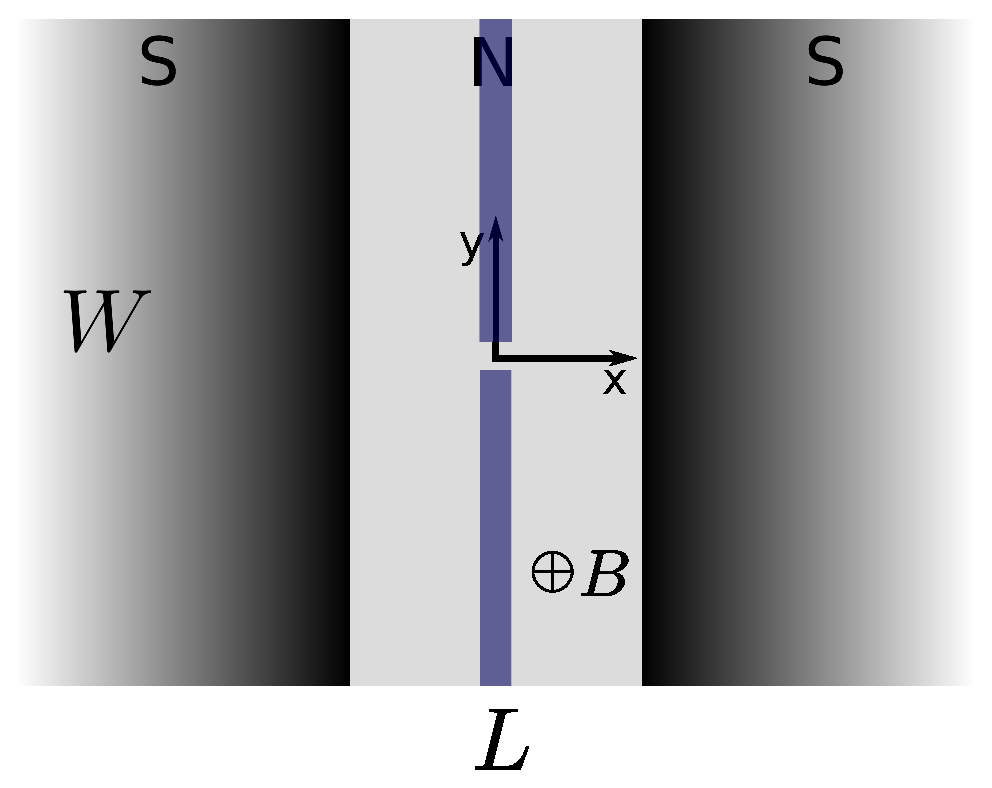
\includegraphics[width=0.6\textwidth]{figure/analyticalmodel/qpc_sns_junction}
\caption{QPC setup.}
\label{fig:qpc_sns_schematic}
\end{figure}
\textbf{TODO: what happens when a constriction is on top of normal layer, fermi levels etc}
The quasiclassical formalism can even be employed to modified SNS junctions. One can build gates on top of the normal region of the junction in a way that the current cannot pass through the gated regions. In the quasiclassical picture, this means that the possibilites for trajectories connecting two points at the superconducting interfaces are limited through the geometry of the constriction.\\
Figure \ref{fig:qpc_sns_schematic} shows a sketch of the quantum point contact setup which will be analysed with the quasiclassical formalism. The normal region of the SNS junction is covered by a gate with a small split in the middle. The split is located at $(x y) = (0, 0)$ so that the sample is symmetric around the origin. The width of the split is in the order of $\lambda_F$ (\textbf{Warum wichtig?}) and can thereby be modeled as an isotropic scattering point with transmission coefficient $\mathcal{T}_0$. Trajectories connecting the two superconducting interfaces have therefore to pass through the QPC. For simplicity the geometrical width of the barrier is neglected and only straight trajectories are considered and scattering at side edges is neglected. This modified setup leads first to a different parametrization of the trajectories and therefore to a different magnetic phase than in eq. (\ref{eq:chi_plane}).\\
With the QPC setup, all possible trajectories are parametrized by two angles $\theta_1$ and $\theta_2$. $\theta_1$ describes the trajectory before passing through the QPC in the region $ -L/2 < x 0$ and  $\theta_2$ after passing through the QPC. The parametrization of the trajectories reads
\begin{equation}
\tan \theta_1 = - \frac{2 y_1}{L}, \quad \tan \theta_2 = \frac{2 y_2}{L}
\label{eq:QPCparametrization}
\end{equation}
With the gauge from eq. (\ref{eq:Ay}) the magnetic phase acquired within the sample reads
\begin{eqnarray}
\frac{2\pi}{\Phi_0} \int d\mathbf{l} \cdot \mathbf{A}  &=&
-\frac{\pi B}{\Phi_0}\left(\frac{L}{2}\right)^2
\left(-\tan\theta_1 + \tan\theta_2\right) =
-\frac{\pi \phi (y_1+y_2)}{2 W}.
\label{eq:phaseQPC}
\end{eqnarray}
Adding this contribution to the term in eq.~(\ref{eq:chi}) the effective phase for the QPC setup is found
\begin{equation}
\tilde{\chi}(y_1,y_2)=\chi-\frac{3 \pi \phi }{2W}(y_1+y_2).
\label{eq:chiQPC}
\end{equation}
The contribution in eq. (\ref{eq:chiQPC}) is half of the effective phase without any constriction, as written in eq. (\ref{eq:chi}). This is reasonable and can be illustrated by looking at the area contributing to the phase. Only half of the normal region is covered by all possible trajectories in the QPC case, whereas in the case without any constriction, the whole normal region contributes.\\
\textbf{TODO: stimmt das da oben? warum?}\\
One consequence of the additional gate on top of the normal region is the change in the effective phase and consequently a modified current phase relation $\mathcal{J}(\tilde{\chi}(y_1, y_2)$. Another consequence is a modified expression for the critical current. In the setup without gates, straight trajectories with a fixed angle $\theta$ were considered and summed up to a total contribution. The difference in the QPC setup is the split in the gate, which is modeled as an isotropic scattering point. The trajectories being summed up in this setup can be thought of two parts. The first part connects $y_1$ with the split at $(x, y) = (0, 0)$ and is determined by the direction of the trajectory. This is why the Fermi velocity enters in this part. The second part of the current trajectory starts from the origin and connects it with a point at the right interface $y_2$. To sum up, the  critical current in the QPC setup is
\begin{equation}
I_c^{\text{QPC}}(\phi) \propto \text{max}_{\chi} \int d \theta_1 v_F \cos^2 \theta_1 \int d \theta_f \cos \theta_f \mathcal{J}\left( \tilde{\chi} (\theta_1, \theta_2) \right)
\end{equation}
%The normalized critical current reads
%\begin{eqnarray}
%\frac{I_c(\phi)}{I_c(0)} &=& \frac{ \text{max}_{\chi} \int d \theta_i \cos^2 \theta_i\int d \theta_f \cos \theta_f \mathcal{J}(\tilde{\chi}(\theta_i, \theta_f)) }{ \text{max}_{\chi} \int d \theta_i \cos^2 \theta_i\int d \theta_f \cos \theta_f \mathcal{J}(\chi) }
%\end{eqnarray}
The QPC is modeled as an isotropic scatterer with transmission probability $\mathcal{T}$. If the transmission is small, $\mathcal{T} << 1$, eq.~(\textbf{TODO: add reference and add formula}) can be used for $\mathcal{J}$.
\textbf{TODO: add why from $\sin \tilde{\chi}$ only cosine survives!}
The angles $\theta_{1, 2}$ can be rewritten in terms of $y_{1, 2}$ by using the parametrization from eq.~(\ref{eq:QPCparametrization}). Using this, the normalized critical current can be expressed as
\begin{eqnarray}
\frac{I_c(\phi)}{I_c(0)} &=& \frac{\mathcal{I}_2(\phi)\mathcal{I}_{3/2}(\phi)}{\mathcal{I}_2(0)\mathcal{I}_{3/2}(0)},
\end{eqnarray}
where the integrals $\mathcal{I}$ are defined as
\begin{equation}
\mathcal{I}_k(\phi) = \frac{2}{L}\int_{-W/2}^{+W/2}dy \frac{\cos\left(\frac{3\pi\phi y}{2W}\right)}{\left[1 + \left(\frac{2y}{L}\right)^2 \right]^k}
\label{integral-qpc}
\end{equation}
The current can be evaluated in the limit of small flux $\phi \rightarrow 0$ and in limit of high fields $\phi \rightarrow \infty$. 
At $\phi=0$ the cosine term becomes one leading to the simple expression
\begin{eqnarray}
\mathcal{I}_2(0)\mathcal{I}_{3/2}(0) &=&
\frac{2 W}{\sqrt{L^2+W^2}}\arctan\frac{W}{L} + \frac{2 L W^2}{(L^2+W^2)^{3/2}} \\
&\equiv& \frac{2x}{\sqrt{1 + x^2}} \arctan x + \frac{2 x^2}{\left( 1 + x^2 \right)^{3/2}}, \quad x = W/L
\label{Ic-0}
\end{eqnarray}
The parabolic asymptotics of the critical current at small $\phi$ is found by expanding the cosine factors in the numerator:
\begin{eqnarray}
\frac{I_c(\phi)}{I_{c0}}&\simeq& 1 - \frac{9\pi ^2 \phi^2 }{32} f_0(W/L) \\
f_0(x) &=& \frac{\sqrt{x^2+1} \log \left(\sqrt{x^2+1}+x\right)}{x^3} - \frac{2}{x (x+(x^2+1) \arctan x)} 
\end{eqnarray}
In the opposite limit of high fields, $\phi\to \infty$, we extend the integration in Eq.~(\ref{integral-qpc}) over $y_1$ and $y_2$ to $\pm \infty$ and obtain
\begin{eqnarray}
\frac{I_c(\phi)}{I_{c0}} &=& \frac{\pi^2 \left(1+x^2\right)^{3/2}}{4x\left(x + \left(1+x^2\right)\arctan x\right)}\left(1 + \frac{3 \pi \phi }{4 x} \right) \sqrt{\frac{3 \phi}{2x}}\exp\left(-\frac{3\phi\pi}{2x}\right)
\label{large-phi}
\end{eqnarray}
\textbf{TODO: write this one in pretty}

\newpage
\section{QPC edge current}
Quasiclassical model applied to edge currents.
Parametriztion here:
\begin{eqnarray}
\tan \theta_1 = ~\frac{ W - y_1}{L/2}, \quad \tan \theta_2 = -\frac{W - y_2}{L/2}
\end{eqnarray}
Magnetic phase gain along trajectory:
\begin{eqnarray}
\frac{2 \pi}{\phi_0} \int d \mathbf{l} \cdot \mathbf{A} &=& \frac{2 \pi}{\phi_0} \left( \int A_y(x) |d\mathbf{l}| |\mathbf{e_y}| \sin \theta_1 + \int A_y(x) |d\mathbf{l}| |\mathbf{e_y}| \sin \theta_2  \right)\\
%&=& \frac{2 \pi B}{\phi_0} \left( \int_{-L/2}^{0} \frac{x dx}{\cos \theta_1} \sin \theta_1  + \int_{0}^{L/2} \frac{x dx}{\cos \theta_2} \sin \theta_2 \right) \\
&=&  - \frac{2 \pi B}{\phi_0} \left( \int_{-L/2}^{0} x dx \tan \theta_1 + \int_{0}^{L/2} x dx \tan \theta_2 \right) \\
&=&  - \frac{\pi B}{\phi_0} \frac{L}{2} \left( - \tan \theta_1 + \tan \theta_2 \right) \\
&=& - \frac{\pi B}{\phi_0} \frac{L}{2} \left( -2W + (y_1 + y_2) \right)\\
&=& \pi \Phi -\frac{\pi \Phi }{2 W} (y_1 + y_2)  
\end{eqnarray}
Using
\begin{equation}
\Phi = \frac{\phi}{\phi_0}, \quad \phi = B W L
\end{equation}
Remember contribution from setup without any constriction eq.~(\ref{eq:chi}), adding this up leads to a total phase for the edge transmission
\begin{equation}
\tilde{\chi}(y_1, y_2) = \chi - \frac{3 \pi \Phi}{2\phi_0} (y_1 + y_2) + \pi \Phi 
\end{equation}



